%%%%%%%%%%%%%%%%%%%%%%%%%%%%%%%%%%%%%%%%%%%%%%%%%%%%%%%%%%%%%%%%%%%%%%%%%%%%%%%
%optimization.tex: Detector Optimization
%%%%%%%%%%%%%%%%%%%%%%%%%%%%%%%%%%%%%%%%%%%%%%%%%%%%%%%%%%%%%%%%%%%%%%%%%%%%%%%%
\chapter{Detector Optimization}
\label{optimization_chapter}
%%%%%%%%%%%%%%%%%%%%%%%%%%%%%%%%%%%%%%%%%%%%%%%%%%%%%%%%%%%%%%%%%%%%%%%%%%%%%%%%

We optimized the detectors for a space-like environment.

%%%%%%%%%%%%%%%%%%%%%%%%%%%%%%%%%%%%%%%%%%%%%%%%%%%%%%%%%%%%%%%%%%%%%%%%%%%%%%%%
% TES Bolometer Theory {{{
%%%%%%%%%%%%%%%%%%%%%%%%%%%%%%%%%%%%%%%%%%%%%%%%%%%%%%%%%%%%%%%%%%%%%%%%%%%%%%%%
\section{Bolometers}
\label{sec:tes_bolometer}
%%%%%%%%%%%%%%%%%%%%%%%%%%%%%%%%%%%%%%%%%%%%%%%%%%%%%%%%%%%%%%%%%%%%%%%%%%%%%%%%

Describe how a bolometer works. Power to temperature detector. Need: cartoon. 

Describe TES.  
\begin{figure}[ht!]
\begin{center}
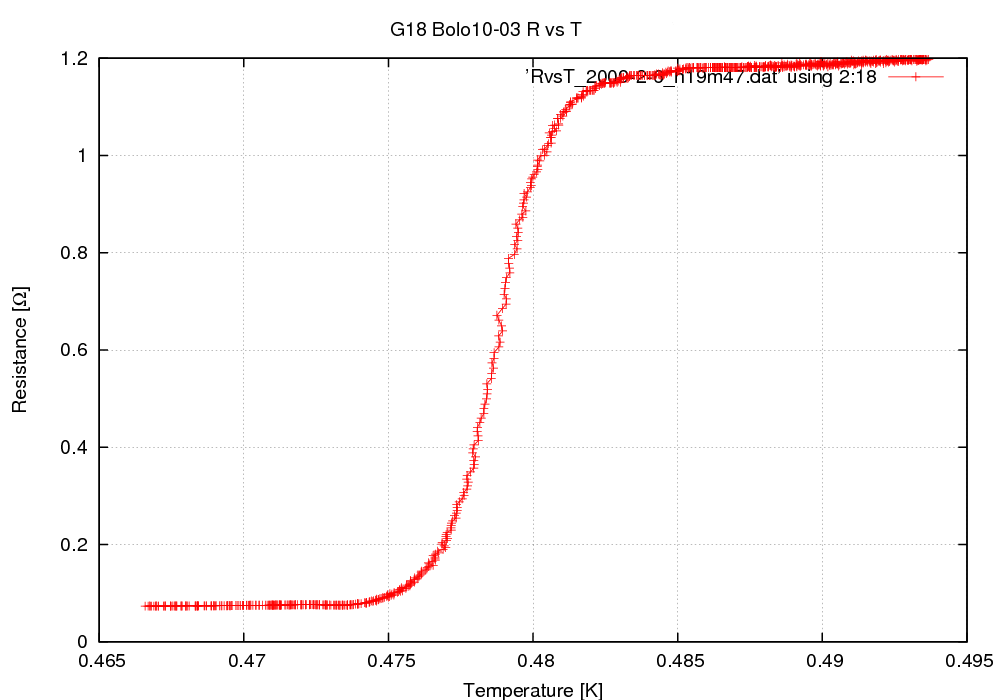
\includegraphics[height=2.5in]{figures/G18_bolo10-03_RvsT_oral}
\caption{Resistance versus temperature for an \ac{EBEX} bolometer.
\label{fig:r_vs_t} }
\end{center}
\end{figure}


Four noise sources, fundamental limit set by photon arrival stats

1. Electronic/Readout

2. Johnson

3. Phonon (ballistic vs �?)

4. Photon (a. Poisson process, b. Shot noise)

%%%%%%%%%%%%%%%%%%%%%%%%%%%%%%%%%%%%%%%%%%%%%%%%%%%%%%%%%%%%%%%%%%%%%%%%%%%%%}}}

